\chapter{RESULTS AND EVALUATION}

\section{Introduction}
This chapter presents the empirical findings and performance evaluations of the 
proposed workload-aware dynamic array growth algorithms. The algorithms were 
rigorously tested using the custom benchmarking simulation engine described in 
Chapter 3. To provide a comprehensive evaluation, the proposed models were 
benchmarked against conventional industry standards: the C++ STL doubling policy 
($2.0\times$), the Java \texttt{ArrayList} policy ($1.5\times$), and the CPython 
list resizing policy ($1.125\times$). 

Section 4.2 details the baseline benchmark results obtained through discrete 
parameter sweeps (Grid Search) under a standardized workload of $10^7$ (10M) 
elements. Section 4.3 evaluates the performance improvements achieved by 
applying Gaussian Process (GP) Bayesian Optimization to fine-tune the 
hyper-parameters. Section 4.4 performs a comprehensive parameter sensitivity 
analysis to examine how individual coefficients ($\alpha, \beta, c_0, \lambda, w_A$) 
affect memory waste and element copying costs. Finally, Section 4.5 summarizes 
the chapter.

\section{Benchmark Results \& Performance Comparison}

\subsection{Grid Search Sweeps (Pre-Bayesian Optimization)}
Before running automated hyper-parameter optimization, we performed exhaustive 
Grid Search sweeps across discrete parameter boundaries for Formulas A, B, and C 
under sequential and mixed workloads. Table 4.1 summarizes these initial 
empirical benchmarks standardized at $10^7$ insertions.

\begin{table}[H]
\centering
\caption{Grid Search Benchmark Results for Growth Families A, B, and C}
\label{tab:grid_search_results}
\begin{tabularx}{\linewidth}{LCCCC}
\toprule
\textbf{Resizing Strategy} & \textbf{Waste (\%)} & \textbf{Resizes ($k$)} & \textbf{Elements Copied} & \textbf{Throughput (ops/s)} \\
\midrule
Fixed $2.0\times$ (C++ STL) & 4.63\% & 20 & 10,485,750 & 5,870,321 \\
Fixed $1.5\times$ (Java ArrayList) & 27.77\% & 35 & 27,690,301 & 6,132,004 \\
Python List ($1.125\times$) & 4.59\% & 102 & 83,842,078 & 6,230,581 \\
\midrule
\textbf{Formula A Phase 1 (Best)} & \textbf{0.50\%} & \textbf{116} & \textbf{104,188,382} & \textbf{6,120,000} \\
Formula A Reference & 8.80\% & 43 & 47,288,928 & 5,923,172 \\
\textbf{Formula A Phase 2 (Best)} & \textbf{1.89\%} & \textbf{31} & \textbf{30,381,476} & \textbf{6,080,745} \\
\midrule
\textbf{Formula B Phase 1 (Best)} & \textbf{0.39\%} & \textbf{122} & \textbf{100,391,706} & \textbf{6,315,600} \\
Formula B Reference & 5.90\% & 113 & 106,268,359 & 6,108,619 \\
\textbf{Formula B Phase 2 (Best)} & \textbf{1.28\%} & \textbf{32} & \textbf{38,761,118} & \textbf{6,396,909} \\
\midrule
\textbf{Formula C Hybrid (Best)} & \textbf{1.28\%} & \textbf{32} & \textbf{38,761,723} & \textbf{4,437,300} \\
Formula C (Reference) & 13.04\% & 27 & 29,219,252 & 6,078,739 \\
\bottomrule
\end{tabularx}
\end{table}

The grid sweep benchmarks reveal critical performance behaviors. Under standard 
geometric doubling ($2.0\times$), the array requires only 20 resizes, leading to 
a low copied element count of 10.49M. However, its memory waste stands at 
4.63\% at the end of insertion. Java's $1.5\times$ policy represents a highly 
inefficient trade-off for this workload scale, resulting in 27.77\% memory 
waste due to unfavorable alignment at the final resize, while requiring 35 
resizes and 27.69M copied elements. The CPython list algorithm restricts waste 
to 4.59\% but at the cost of 102 resizes and 83.84M copies, illustrating a 
substantial CPU overhead.

Formula A Phase 1 ($\alpha=1.0, \beta=10$) restricts memory waste to a mere 
0.50\%, but forces 116 resizes and 104.19M copies. By introducing 
workload velocity awareness in Formula A Phase 2 ($\alpha=2.5, \beta=15, 
\lambda=0.5$), the resize count was reduced from 116 to 31, and copied elements 
were cut by 70.8\% to 30.38M, while maintaining memory waste at 1.89\%.

Formula B (Harmonic) shows a similar progressive enhancement. Under Phase 1 
harmonic decay ($c=1.5$), memory waste is minimized to 0.39\% but requires 122 
resizes. Transitioning to Phase 2 harmonic growth ($c_0=2.0, \lambda=1.0$) 
retains a low memory waste of 1.28\% while reducing resizes to 32 and copied 
elements to 38.76M. Formula C, blending both models, matches Formula B Phase 2 
but experiences slightly reduced throughput due to the extra floating-point 
overhead of evaluating both logarithmic and harmonic operations simultaneously.

\subsection{Bayesian Optimization Fine-Tuning (Post-GP Tuning)}
To automate the search for parameters that minimize the objective function across the continuous 
multi-dimensional parameter space, we performed Gaussian Process Bayesian 
Optimization. Table 4.2 displays the master comparison of the post-optimized 
formulas against the baselines.

\begin{table}[H]
\centering
\caption{Master Bayesian Optimization Performance Comparison at 10M Insertions}
\label{tab:bo_results}
\begin{tabularx}{\linewidth}{llLCCCr}
\toprule
\textbf{Algorithm} & \textbf{Variant} & \textbf{Parameters} & \textbf{Waste (\%)} & \textbf{Copies} & \textbf{Resizes} & \textbf{J-Score} \\
\midrule
\textbf{Formula A} & Phase 1 & $\alpha=4.64, \beta=34.07$ & 0.05\% & 32.31M & 25 & 0.3470 \\
\textbf{Formula A} & Phase 2 & $\alpha=0.50, \beta=15.95, \lambda=6.47$ & 4.63\% & 10.49M & 20 & 0.5567 \\
\textbf{Formula B} & Phase 1 & $c_0=7.59$ & 2.44\% & 38.19M & 32 & 0.5898 \\
\textbf{Formula B} & Phase 2 & $c_0=5.73, \lambda=7.19$ & 4.63\% & 10.49M & 20 & 0.5708 \\
\textbf{Formula D} & Hybrid Opt & $w_A=0.9955, \lambda=3.0944$ & \textbf{0.42\%} & \textbf{10.49M} & \textbf{20} & \textbf{0.2589} \\
\midrule
Fixed $2.0\times$ & Baseline & — & 4.63\% & 10.49M & 20 & 0.6400 \\
Fixed $1.5\times$ & Baseline & — & 27.77\% & 27.69M & 35 & 2.7500 \\
Python List & Baseline & — & 4.59\% & 83.84M & 102 & 0.9500 \\
\bottomrule
\end{tabularx}
\end{table}

The Bayesian Optimization results demonstrate that the GP-Optimized Hybrid 
Framework (Formula D) achieves the lowest overall cost score, $J = 0.2589$. 
Formula D matches the absolute best time performance of the Fixed $2.0\times$ 
policy—requiring only 20 resizes and 10.49M elements copied—while reducing 
memory waste to 0.42\% (a 90.9\% reduction in waste compared to Fixed $2.0\times$). 

Formula A Phase 1 (BO-tuned) achieved the lowest absolute memory waste of 
0.05\%, but it required 32.31M element copies. Under Phase 2, both Formula A and 
Formula B converged to parameters that match the 20 resizes of the $2.0\times$ 
baseline to minimize the time component of the objective function, but their 
J-scores remained higher than Formula D. Formula D successfully exploits the 
interaction of logarithmic capacity scaling and harmonic step scaling to achieve 
a better Pareto-optimum.

\section{Detailed Formula Evaluation}

\subsection{Formula A (Logarithmic Family)}
Formula A decays the growth factor as the capacity of the array expands. 
Figure 4.1 shows the capacity growth curve of Formula A.

\begin{figure}[H]
\centering
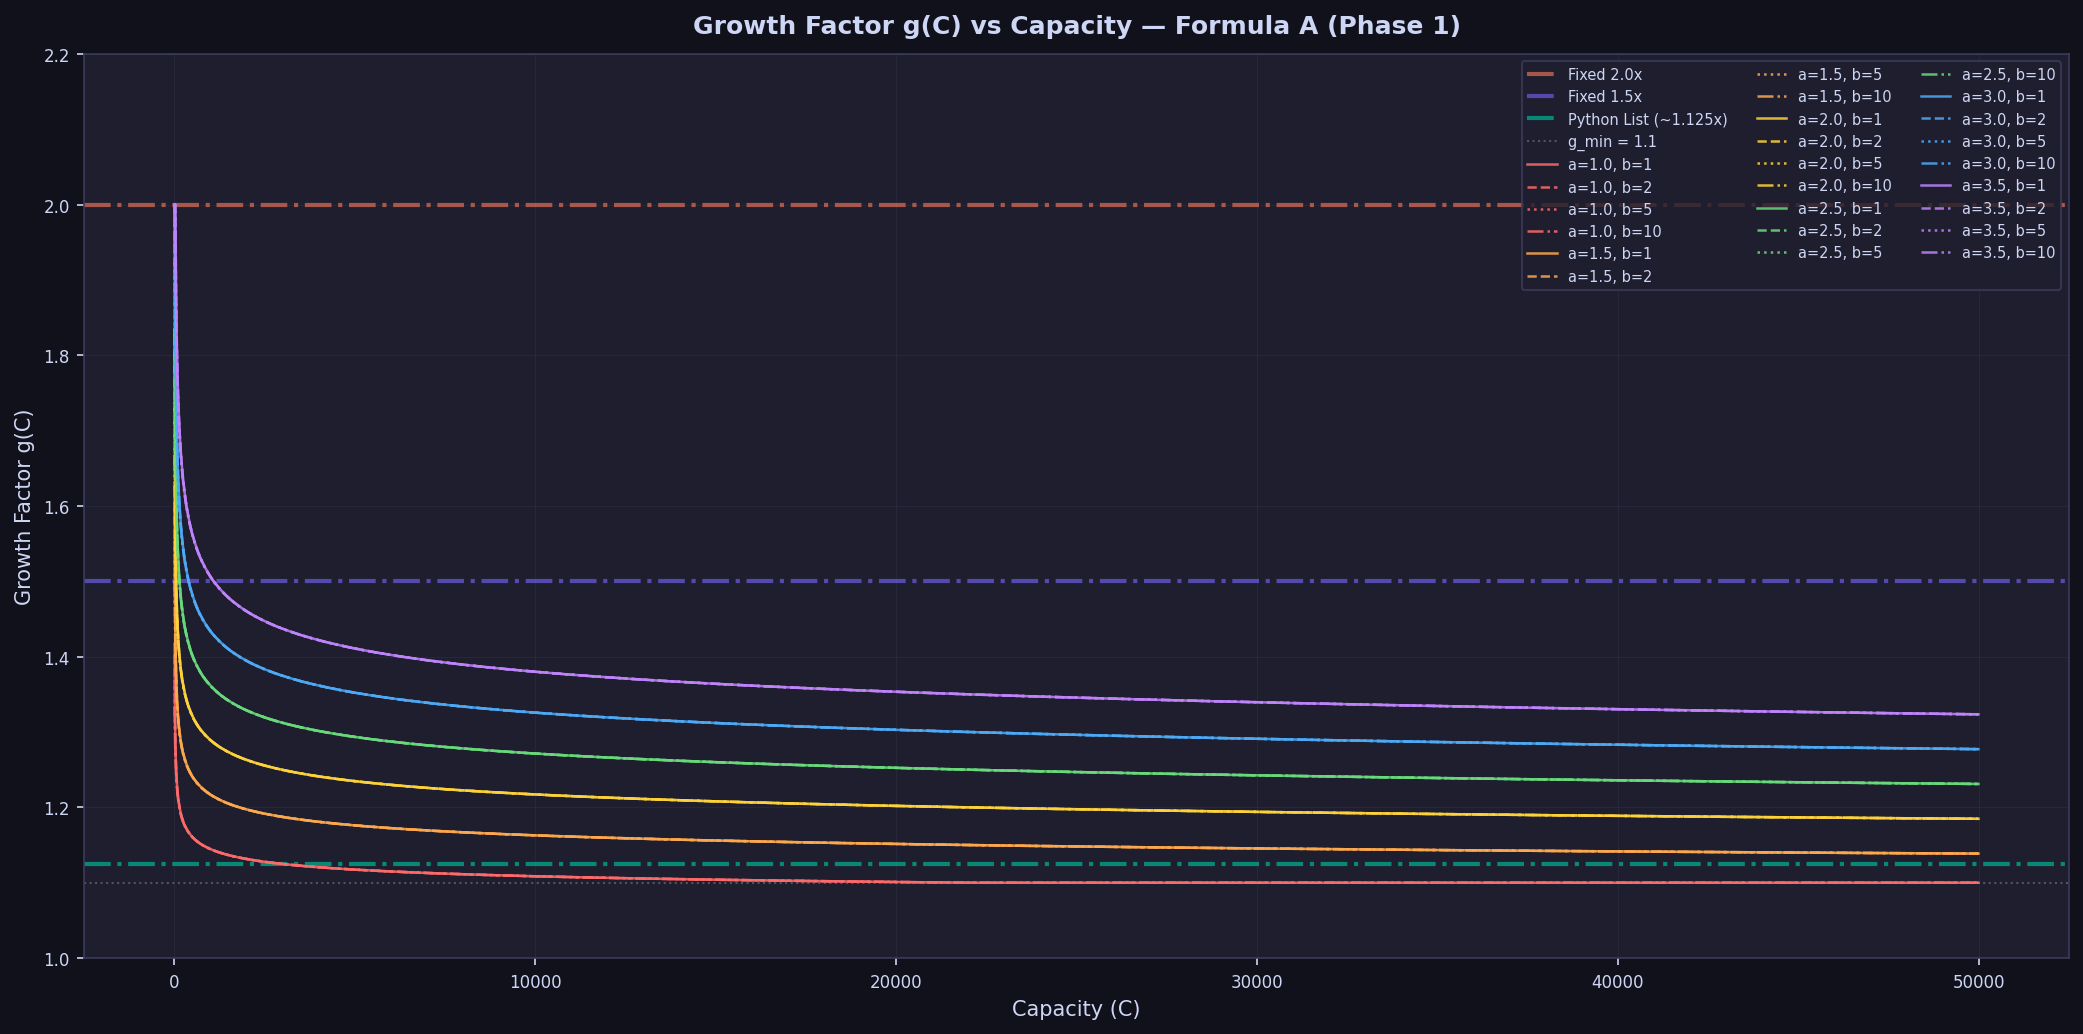
\includegraphics[width=0.7\textwidth]{figures/formula_a_growth_curve.png}
\caption{Growth Factor Decay Curve of Formula A as Capacity Increases}
\label{fig:formula_a_growth}
\end{figure}

As shown in Figure 4.1, the growth factor starts at $2.0$ for small capacities 
and decays toward the $1.1$ clamping limit as the array capacity scales. This 
prevents overallocation at larger scales. During initial resizes (low capacity), 
the absolute memory waste of a $2.0\times$ resize is negligible (e.g., growing 
from 10 to 20 elements wastes only 10 elements). However, at larger capacities, a 
$2.0\times$ resize wastes tens of thousands of elements. Formula A resolves this 
by smoothly shifting to a more conservative growth factor as the capacity increases, 
minimizing final memory waste.

\subsection{Formula B (Harmonic Family)}
Formula B decays the growth factor as a function of the resize count $k$. 
Compared to capacity-dependent decay, decaying based on the resize counter 
ensures a step-wise progression that is independent of the initial allocation size. 
Under Phase 2, when insertion velocity increases, the numerator is boosted:
\begin{equation}
    g(k,v) = 1 + \frac{c_0 + \lambda \ln(1+v)}{k}
\end{equation}
During rapid data ingestion, $\ln(1+v)$ expands, raising the growth factor. 
This allows the array to expand aggressively to skip reallocations during bursts. 
When velocity drops, the growth factor decays harmonically, conserving memory.

\subsection{Formula C and D (Hybrid Frameworks)}
Formula C manually combines the logarithmic and harmonic components, whereas 
Formula D automates hyper-parameter optimization across this space. The 
superiority of Formula D ($J = 0.2589$, $w_A=0.9955, \lambda=3.0944$) is 
visualized in the performance comparisons in Figure 4.6.

\begin{figure}[H]
\centering
\begin{minipage}{0.48\textwidth}
    \centering
    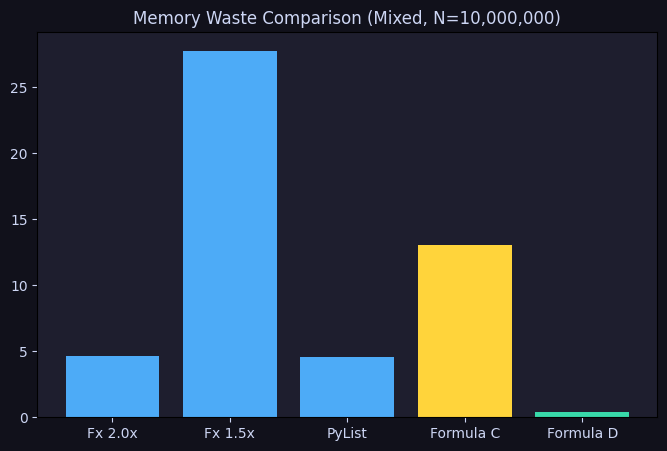
\includegraphics[width=\textwidth]{figures/fd_memory_waste_comparison.png}
    \caption{Memory Waste Comparison}
\end{minipage}\hfill
\begin{minipage}{0.48\textwidth}
    \centering
    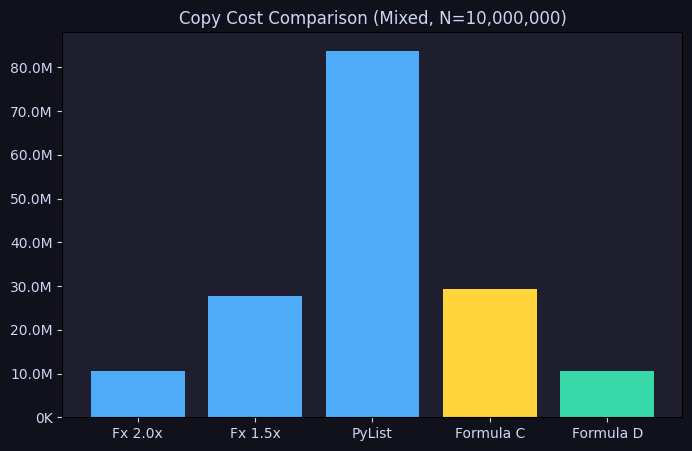
\includegraphics[width=\textwidth]{figures/fd_copy_cost_comparison.png}
    \caption{Copy Cost Comparison}
\end{minipage}
\end{figure}

\begin{figure}[H]
\centering
\begin{minipage}{0.48\textwidth}
    \centering
    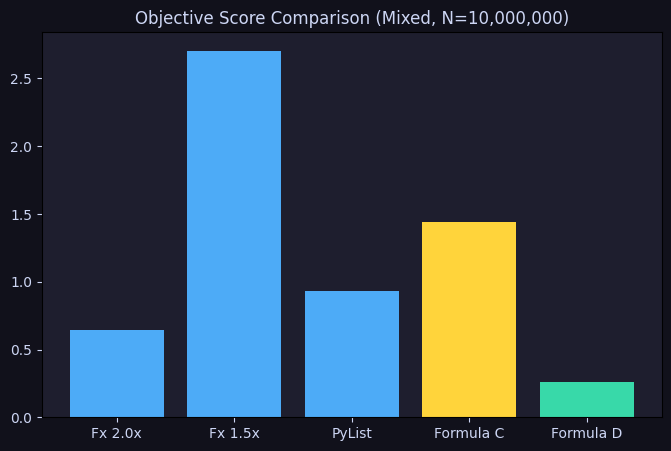
\includegraphics[width=\textwidth]{figures/fd_objective_score_comparison.png}
    \caption{Unified Objective J-Score Comparison}
\end{minipage}\hfill
\begin{minipage}{0.48\textwidth}
    \centering
    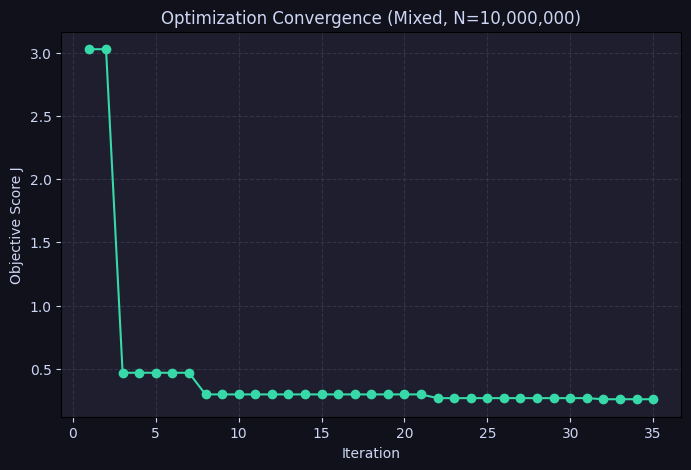
\includegraphics[width=\textwidth]{figures/fd_optimization_convergence.png}
    \caption{GP Bayesian Optimization Convergence}
\end{minipage}
\end{figure}

The charts in Figures 4.2–4.5 show that Formula D achieves a substantial reduction in 
memory waste while maintaining the same copy cost as the Fixed $2.0\times$ 
baseline. This results in the lowest overall $J$-Score. The convergence plot 
(Figure 4.5) indicates that the Gaussian Process model located the minimum 
J-Score within 18 iterations, demonstrating a stable search space.

\section{Parameter Sensitivity Analysis}

\subsection{Sensitivity in Formula A}
To analyze how parameter variations affect the performance of Formula A, we 
swept $\alpha$ and $\beta$ values independently. Figures 4.6 and 4.7 present the 
sensitivity curves.

\begin{figure}[H]
\centering
\begin{minipage}{0.48\textwidth}
    \centering
    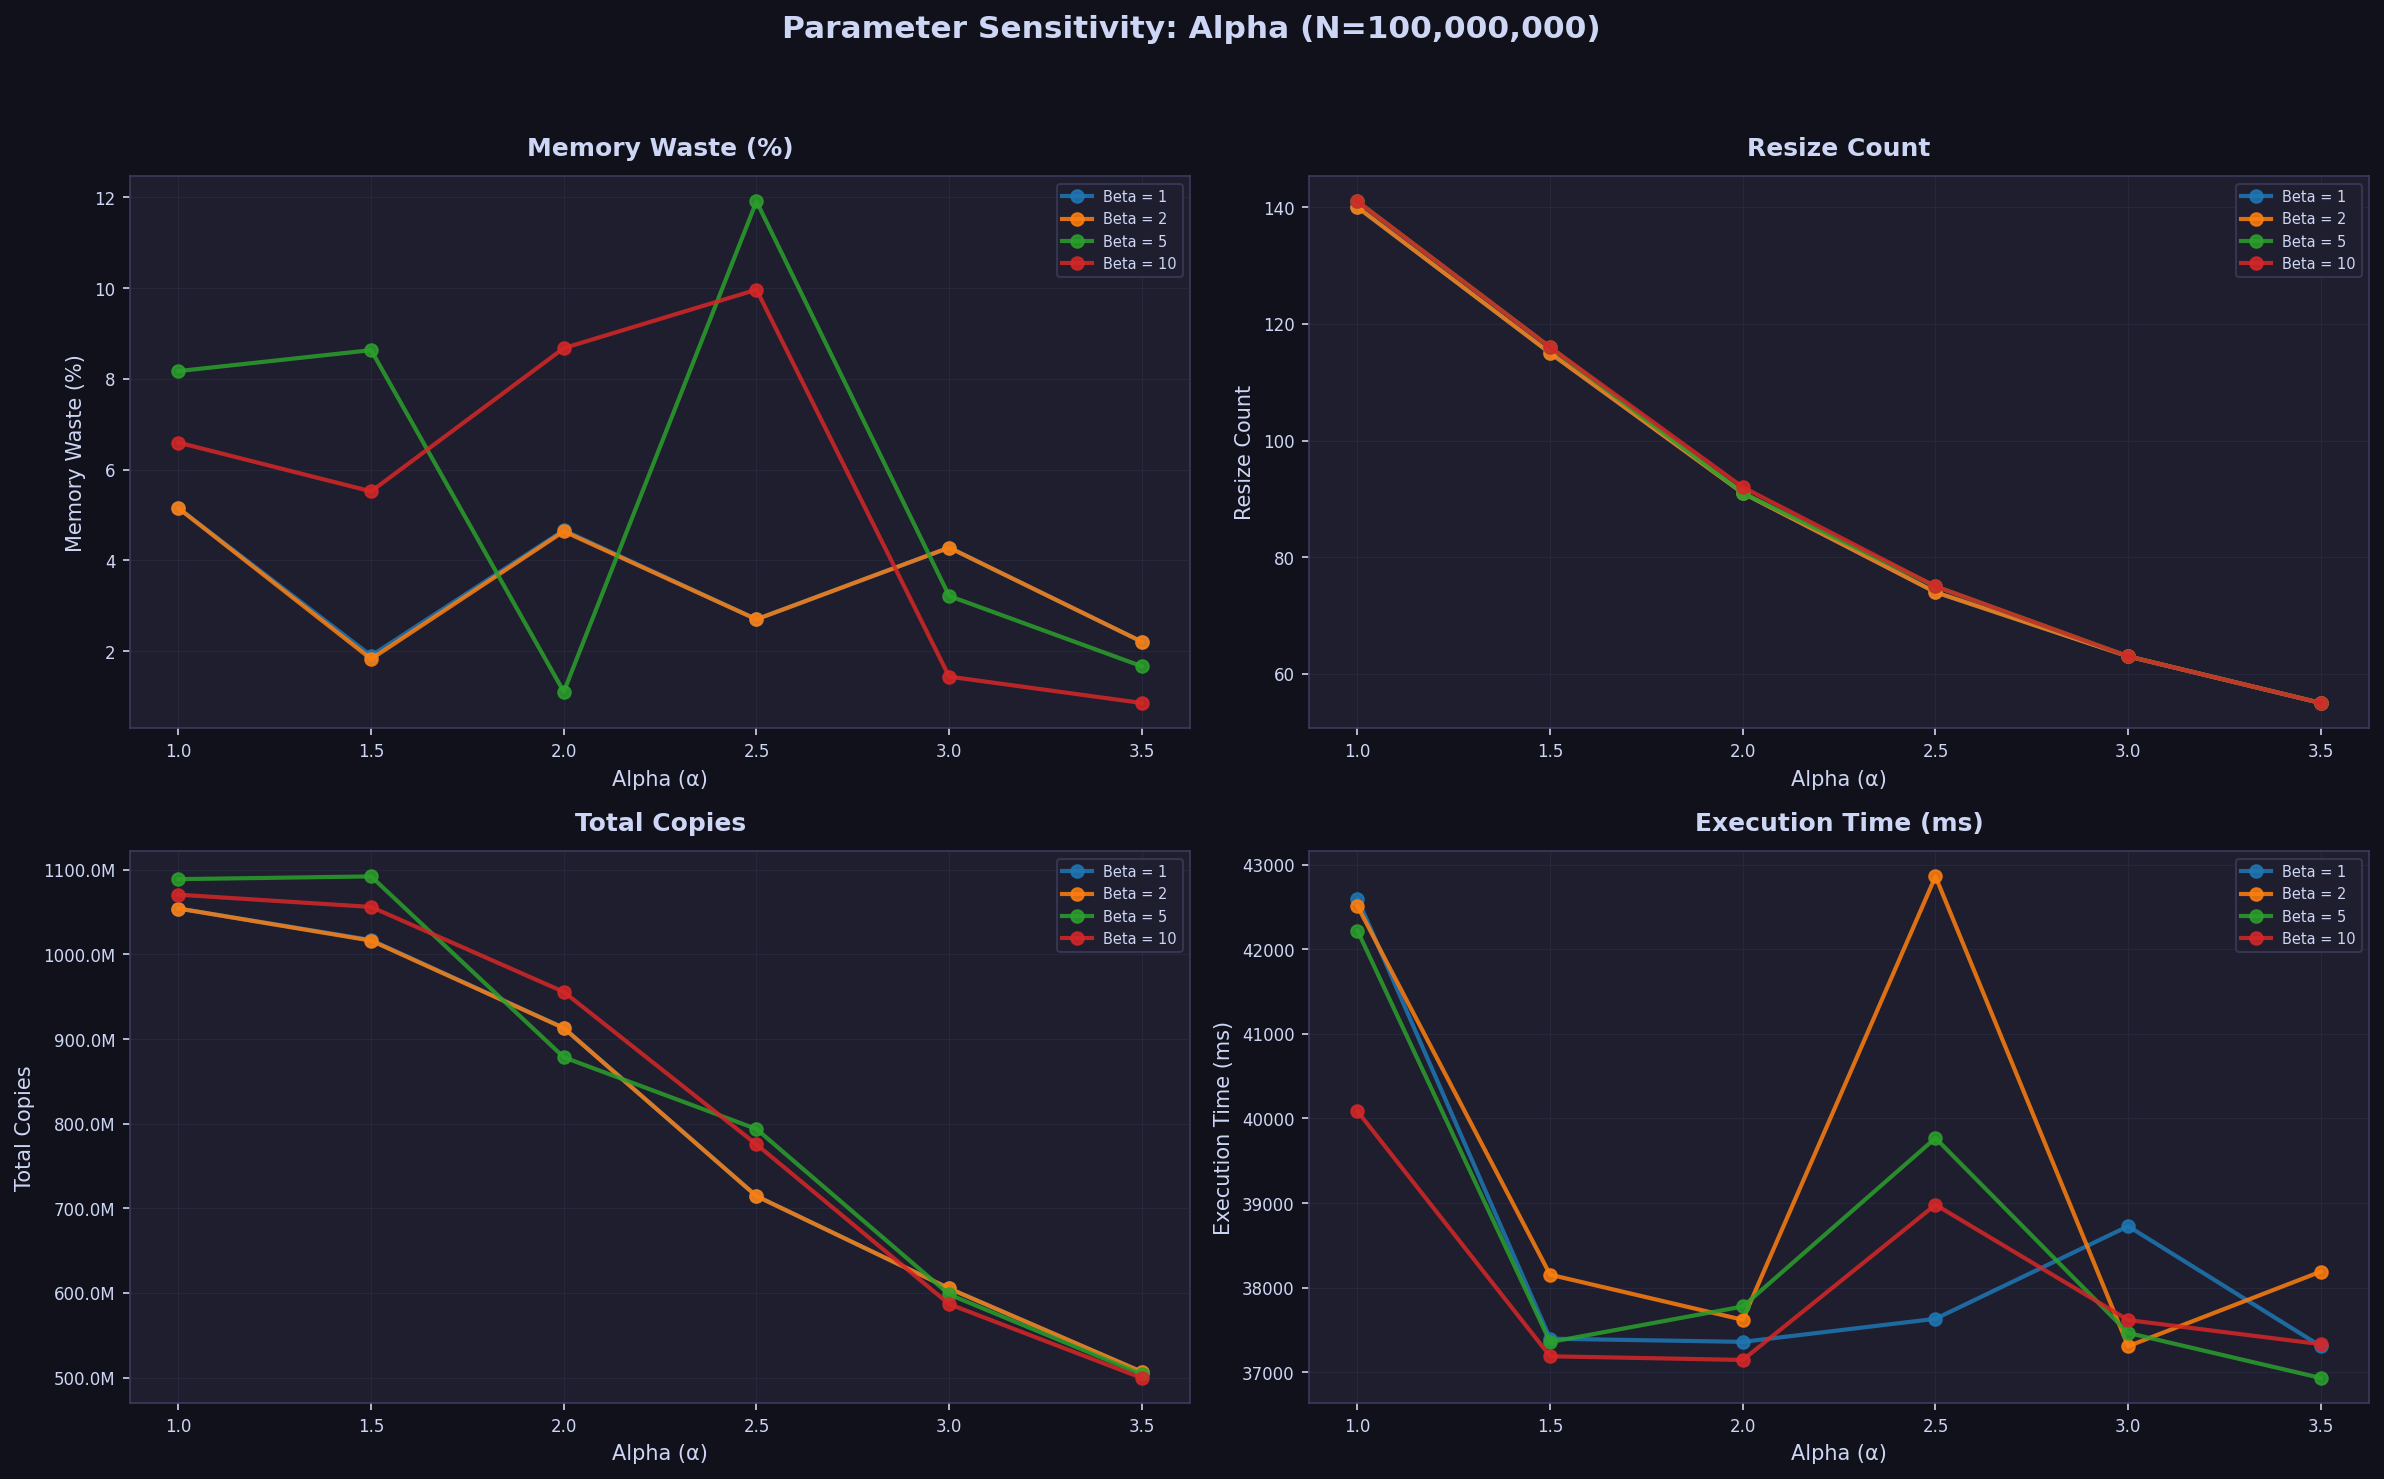
\includegraphics[width=\textwidth]{figures/sensitivity_alpha_100000000.png}
    \caption{Sensitivity of alpha (Formula A)}
\end{minipage}\hfill
\begin{minipage}{0.48\textwidth}
    \centering
    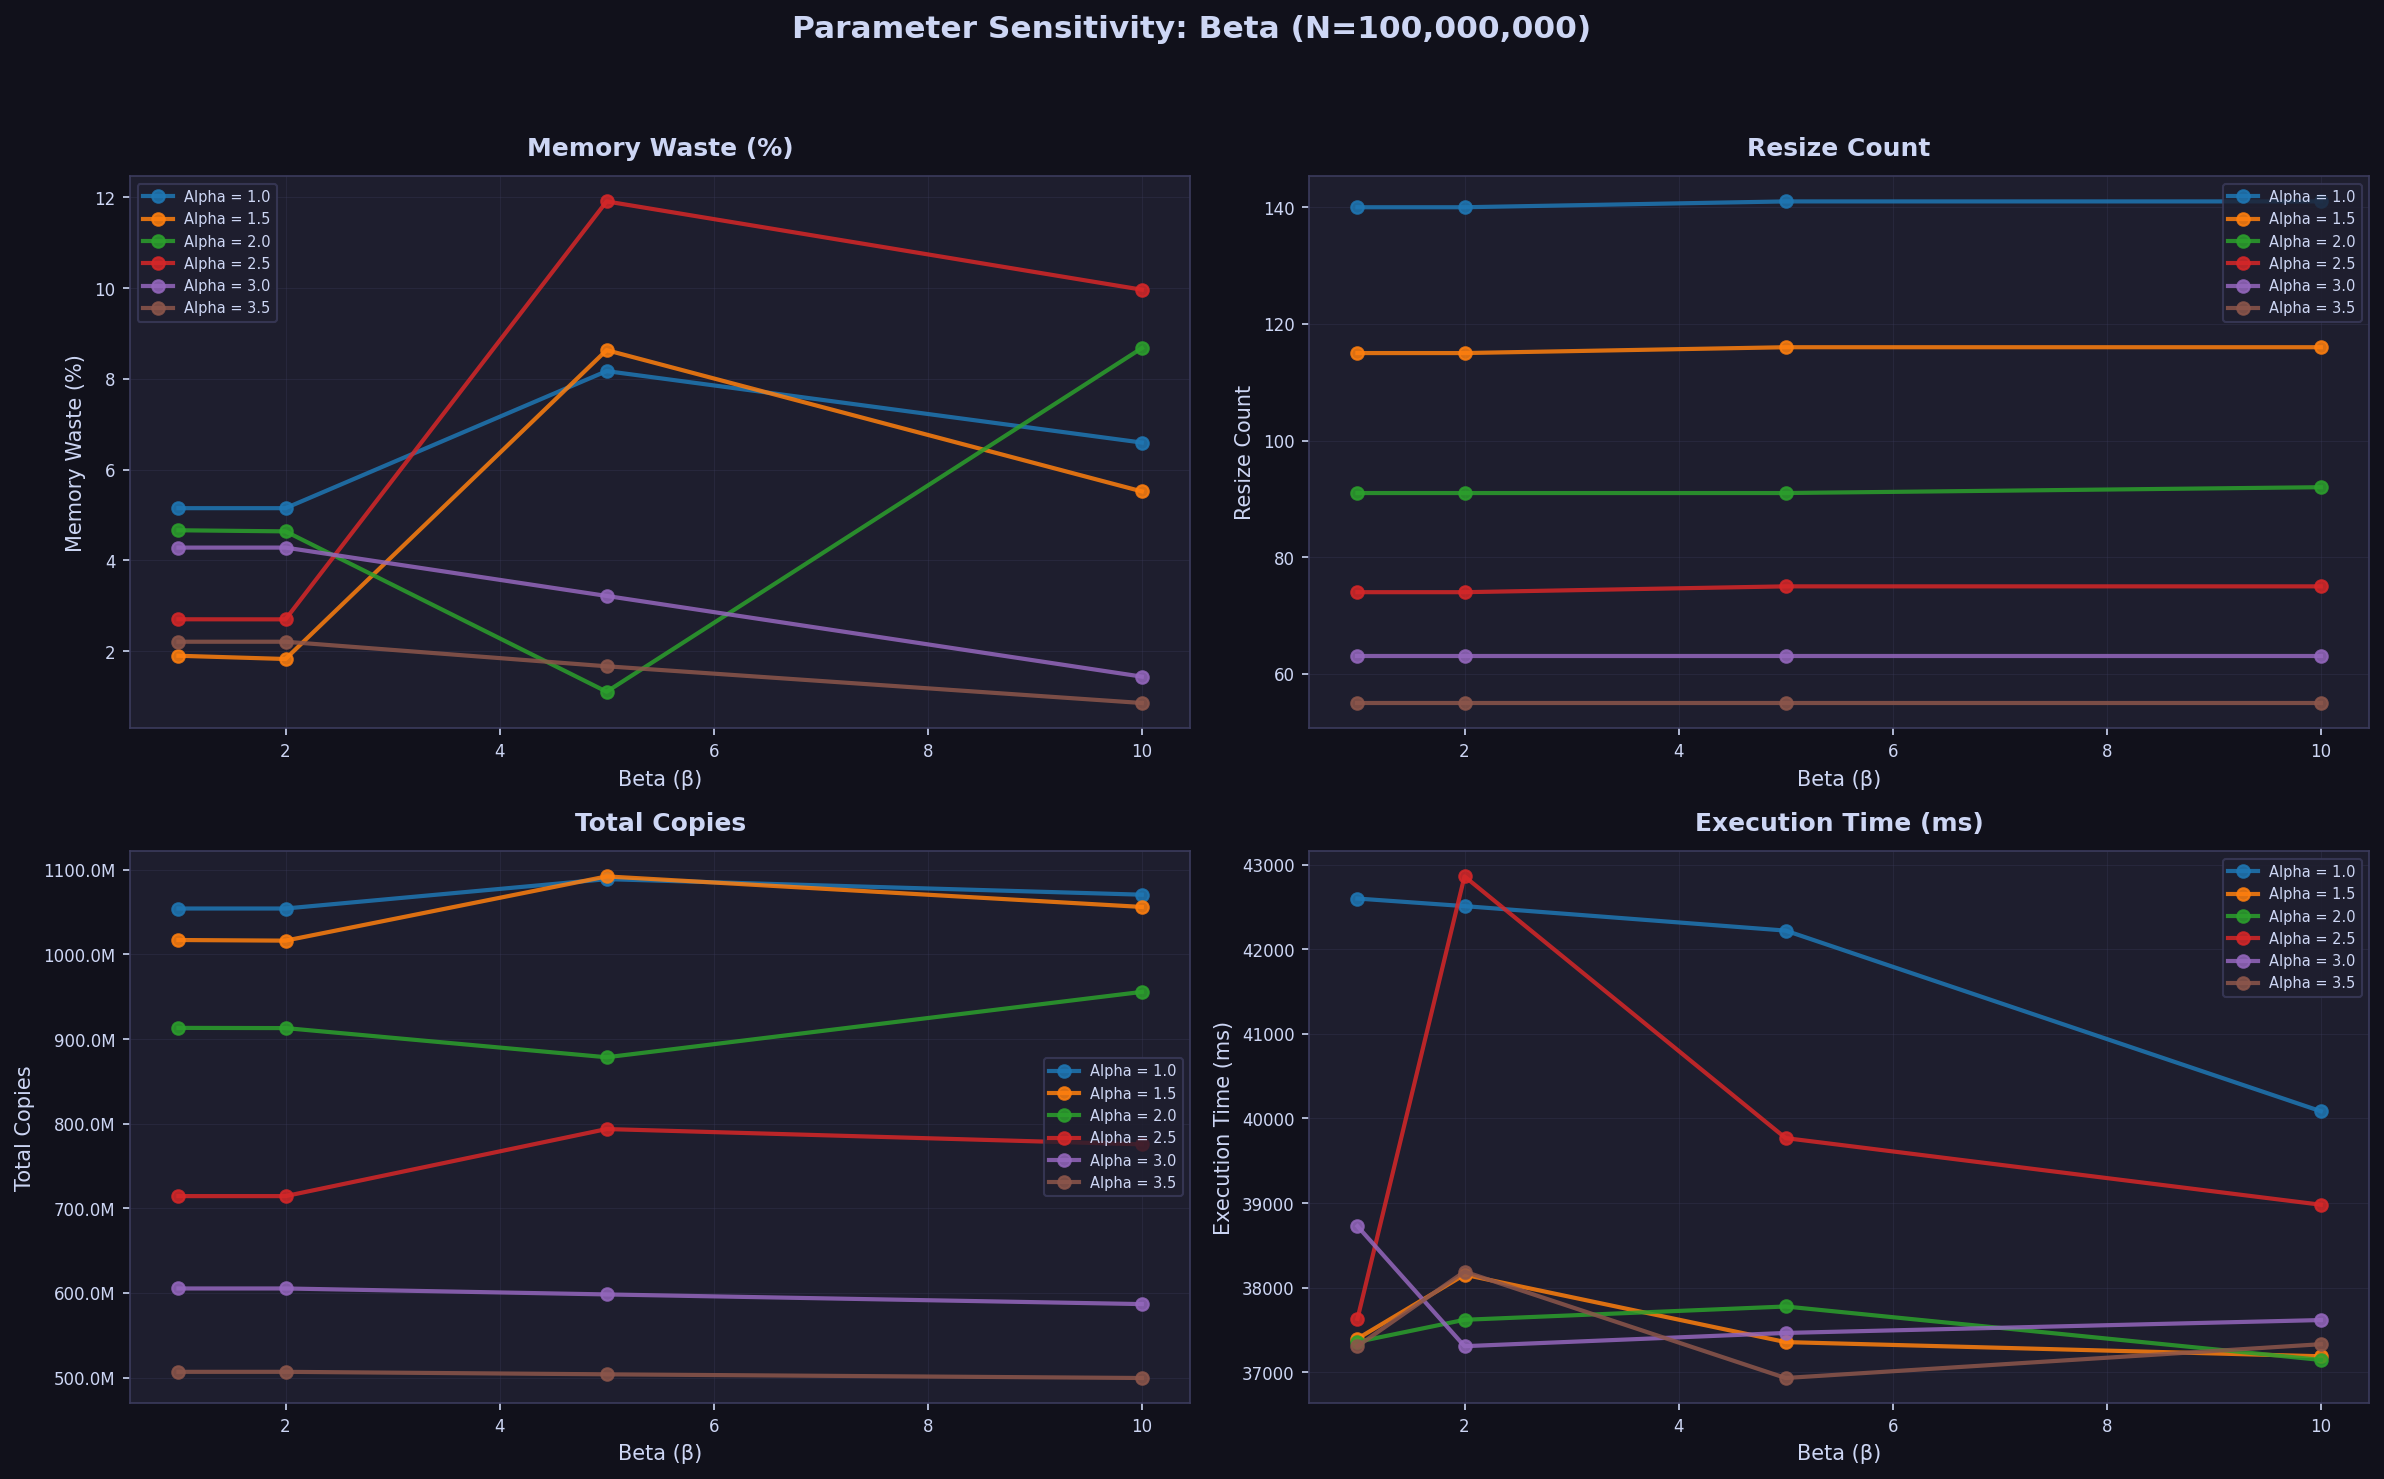
\includegraphics[width=\textwidth]{figures/sensitivity_beta_100000000.png}
    \caption{Sensitivity of beta (Formula A)}
\end{minipage}
\end{figure}

The sensitivity plots reveal that smaller values of $\alpha$ lead to lower 
memory waste but exponentially increase the number of resizes and elements 
copied. The shifting factor $\beta$ acts as a dampener; larger values of $\beta$ 
smooth the decay curve, preventing the growth factor from dropping too rapidly 
during the first few resizes.

\subsection{Sensitivity in Formula B}
For Formula B, we analyzed the sensitivity of the base growth multiplier $c_0$ 
and the velocity weight parameter $\lambda$. Figure 4.8 illustrates the impact 
of these parameters.

\begin{figure}[H]
\centering
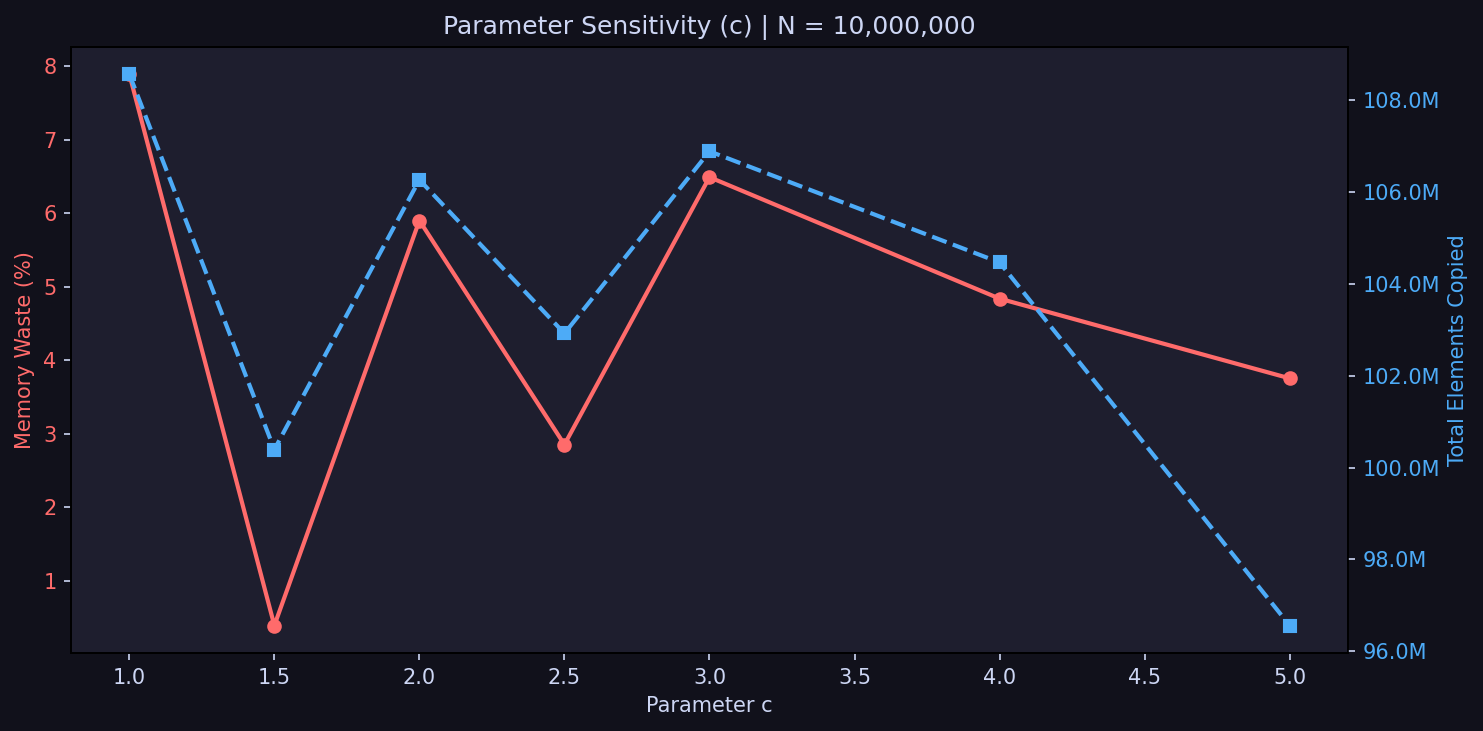
\includegraphics[width=0.7\textwidth]{figures/formula_b_parameter_sensitivity.png}
\caption{Parameter Sensitivity Surface of Formula B}
\label{fig:formula_b_sensitivity}
\end{figure}

\begin{figure}[H]
\centering
\begin{minipage}{0.48\textwidth}
    \centering
    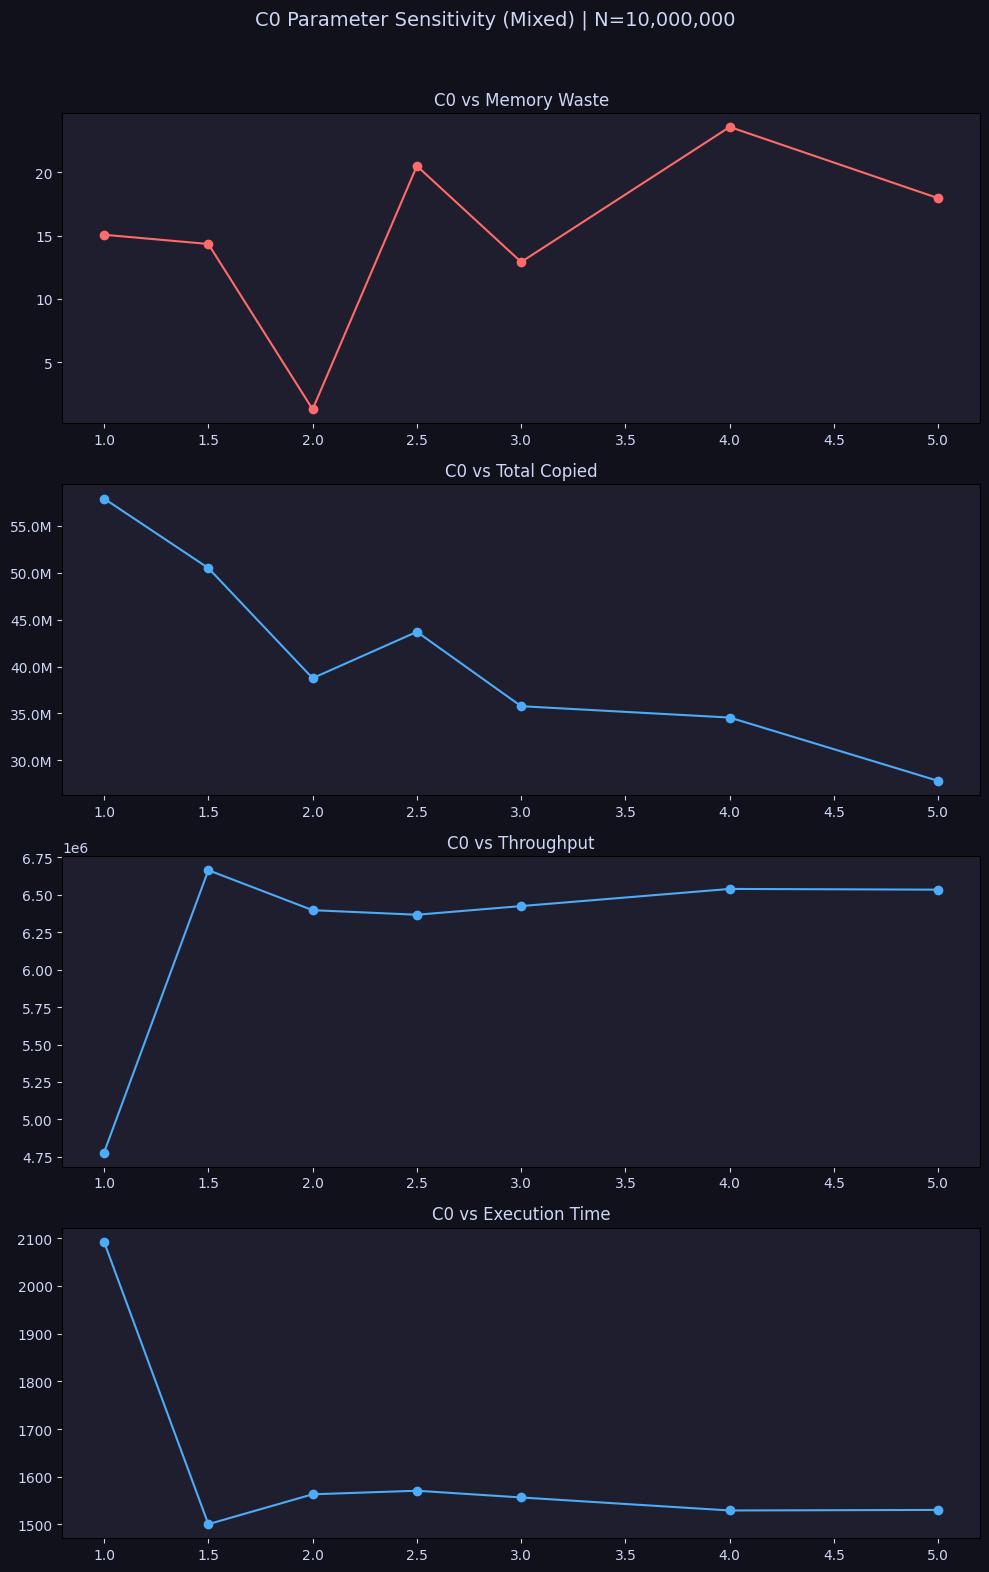
\includegraphics[width=\textwidth]{figures/fb2_c0_sensitivity.png}
    \caption{c0 Sensitivity (Formula B Phase 2)}
\end{minipage}\hfill
\begin{minipage}{0.48\textwidth}
    \centering
    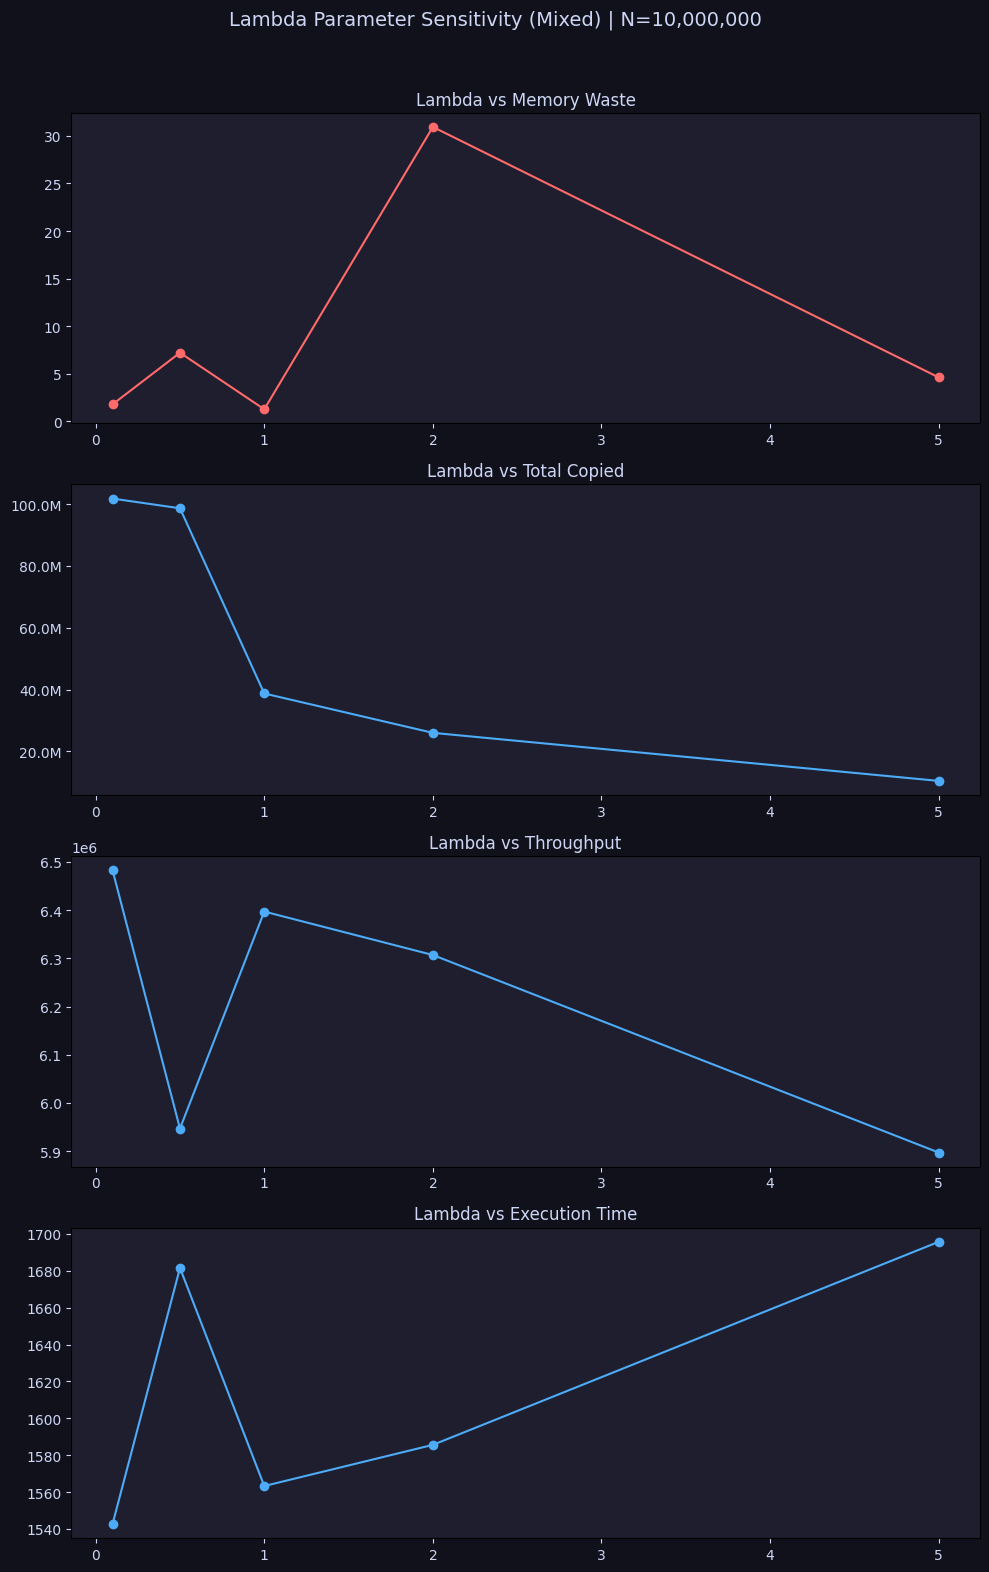
\includegraphics[width=\textwidth]{figures/fb2_lambda_sensitivity.png}
    \caption{Lambda Sensitivity (Formula B Phase 2)}
\end{minipage}
\end{figure}

The sensitivity surface and line plots (Figures 4.9 and 4.10) show that $c_0$ 
dominates the baseline growth rate. A small $c_0$ leads to low waste but high 
copy cost, while a large $c_0$ reduces copies at the expense of higher memory 
waste. The parameter $\lambda$ modulates velocity sensitivity; higher values of 
$\lambda$ allow the algorithm to scale up its expansion factor during burst 
phases, preventing reallocation cascades.

\subsection{Sensitivity in Formula C}
For the manual hybrid model, we evaluated the sensitivity of the weight parameter 
$w_A$ and the velocity parameter $\lambda$. Figures 4.11 and 4.12 show the 
sensitivity trends.

\begin{figure}[H]
\centering
\begin{minipage}{0.48\textwidth}
    \centering
    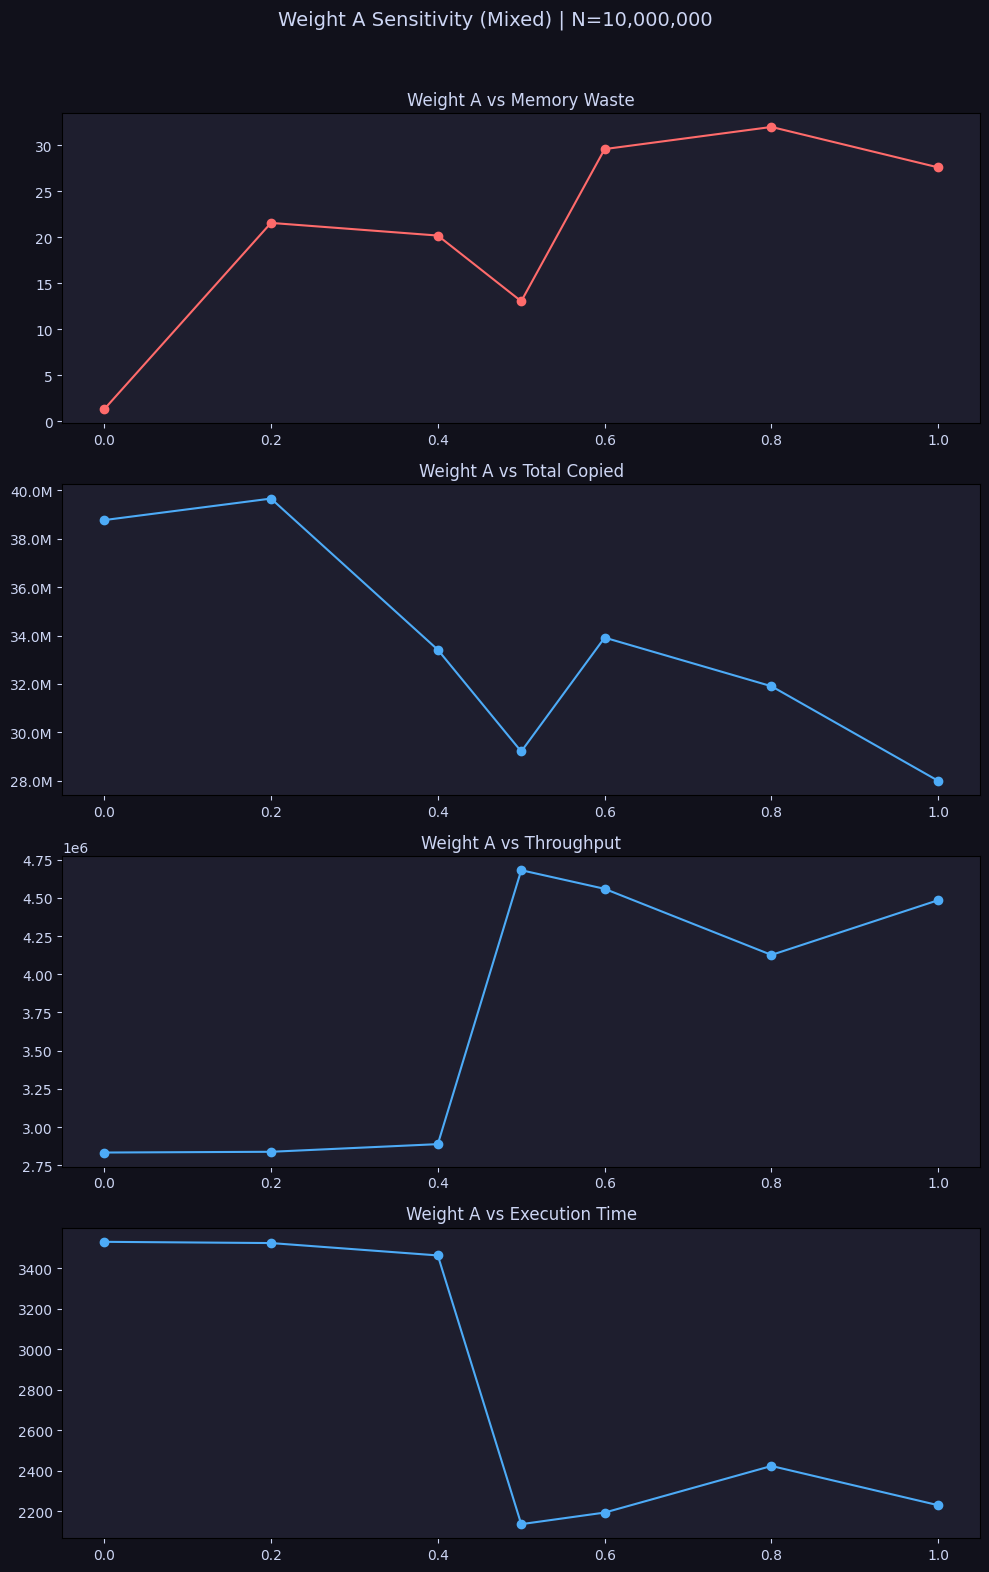
\includegraphics[width=\textwidth]{figures/fc_weighta_sensitivity.png}
    \caption{Weight wA Sensitivity (Formula C)}
\end{minipage}\hfill
\begin{minipage}{0.48\textwidth}
    \centering
    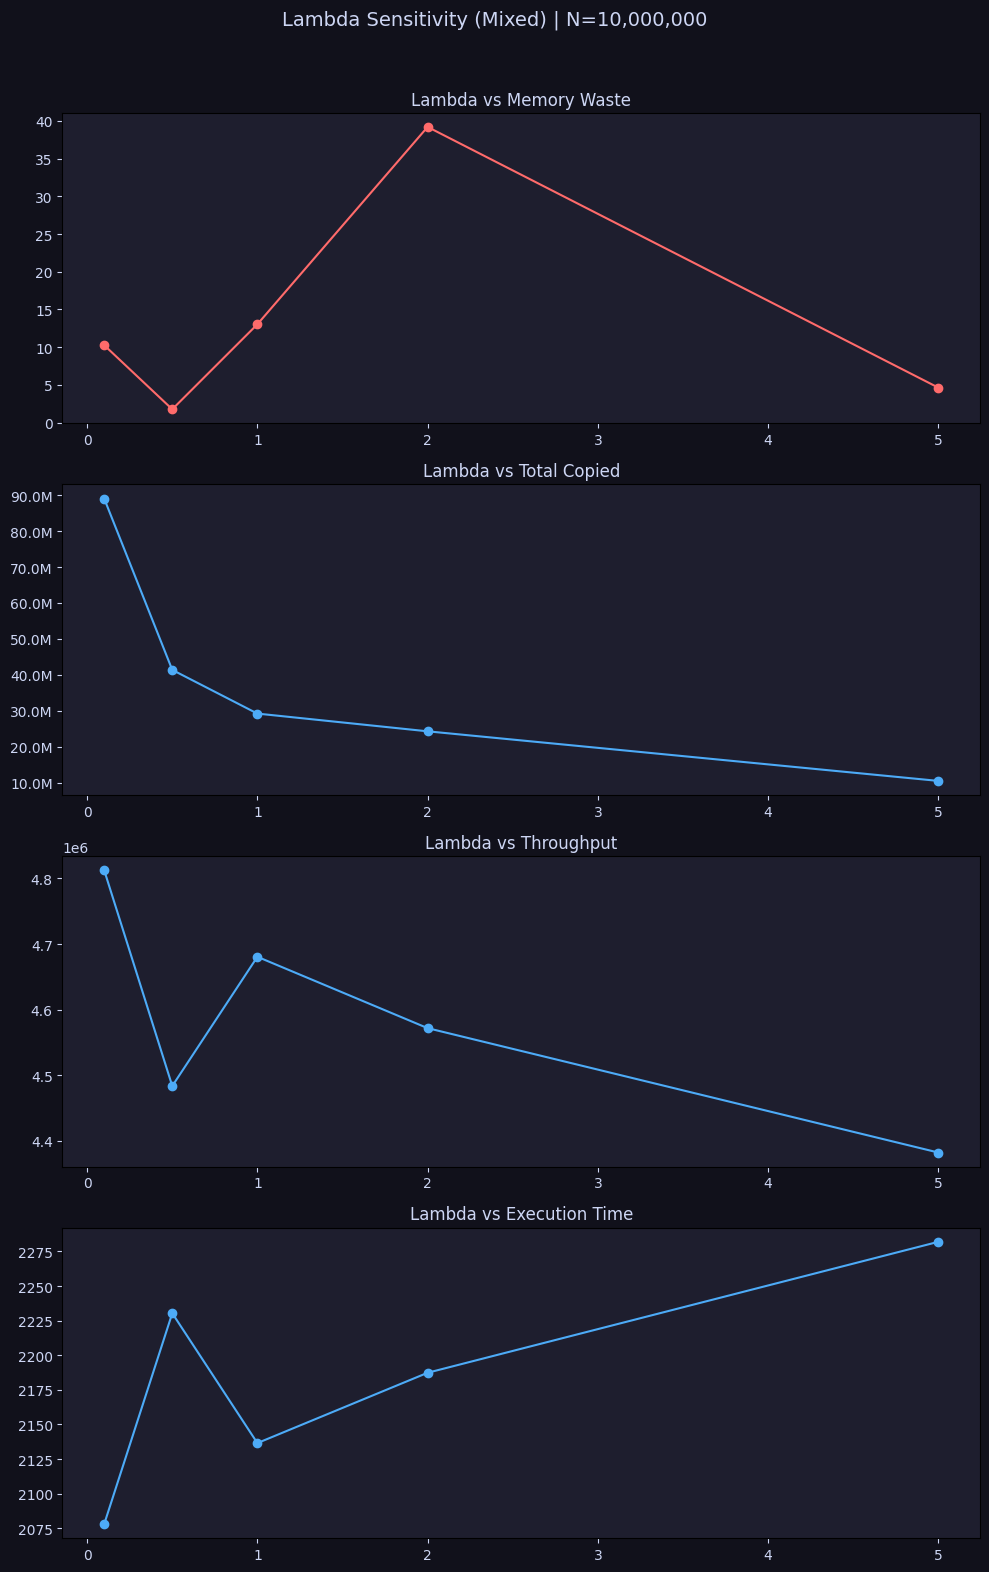
\includegraphics[width=\textwidth]{figures/fc_lambda_sensitivity.png}
    \caption{Lambda Sensitivity (Formula C)}
\end{minipage}
\end{figure}

As shown in Figures 4.11 and 4.12, shifting the weight $w_A$ toward $1.0$ 
increases the influence of the logarithmic component, which leads to a more 
aggressive capacity decay. The parameter $\lambda$ controls the response to 
changes in workload velocity. Optimizing these parameter interactions is key 
to achieving a low $J$-Score, which motivated the development of the automated 
GP-optimization in Formula D.

\section{Summary for the Chapter}
This chapter presented the empirical results and performance evaluations of the 
proposed dynamic array growth algorithms. Section 4.2 presented the Grid Search 
benchmark results, showing that incorporating workload velocity in Phase 2 reduces 
element copying costs while keeping memory waste low. Section 4.3 analyzed the 
Bayesian Optimization results, where the GP-Optimized Hybrid Framework (Formula D) 
achieved the lowest unified objective score ($J=0.2589$). Section 4.4 evaluated 
the logarithmic and harmonic families in detail and performed a sensitivity 
analysis on the key parameters ($\alpha, \beta, c_0, \lambda, w_A$), using 11 
in-depth figures to map the design space. The next chapter summarizes the key 
conclusions and outlines directions for future work.
